\chapter{Example}
\label{example}
\pagenumbering{arabic}
\setcounter{page}{19}



A simulated XRD pattern for LiNiO$_{2}$ has been used to analyse and test out the program. 
The initial values of the refinement have been chosen far enough from the correct ones not to bias the result.
The refinement has  been carried out using the Levenberg-Marquardt fit. 


\section{Stacking faults in LiNiO$_{2}$}

Lithium nickel oxide has been intensively studied as a positive electrode material in Li-ion batteries \cite{Whit2004}. 
As other lithium transition metal oxides it presents an O3-type layered structure, consisting in three NiO$_{2}$ slabs per unit cell with an ABCABC oxygen stacking sequence and lithium ions located in the octahedral sites of the interlayer spaces (see figure \ref{estructura}). In order to explain the significant broadening of the (10l) and (01l) diffraction lines, DIFFaX simulations have been used for this material with the hypothesis of the existence of O1 stacking faults in the structure \cite{Crog2000}. These stacking faults represent a break in the normal stacking sequence of the structure, with a local ABAB oxygen stacking sequence.

\begin{figure}[!htbp]
\begin{center}
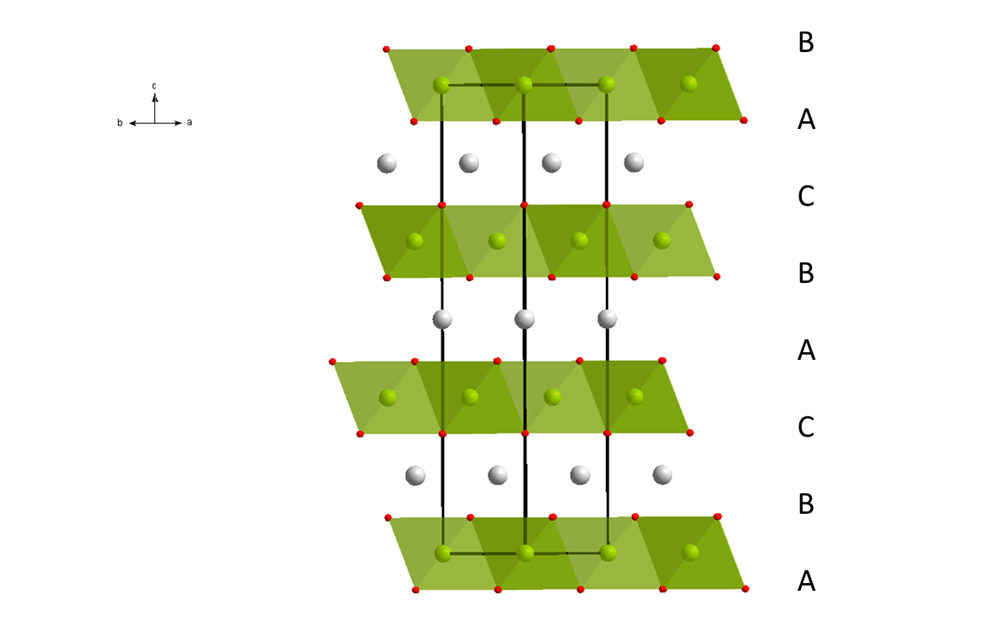
\includegraphics [width=4 in]{LiNO_estructura.png}
\caption{\bf Structure of lithium nickel oxide (LiNiO$_{2}$).}
\label{estructura}
\end{center}
\end{figure}

The ideal structure can be described with three layers, each one containing a NiO$_{2}$ slab and a lithium sheet. The three layers are structurally identical, but shifted with respect to each other, resulting in transition vectors $\vec{t}$12=$\vec{t}$23=$\vec{t}$31=(2/3 1/3 1/3) and a stacking probability of 1 for each transition. O1 defects require the definition of a new type of layer, structurally differente, since the position of Li atoms will be different (see figure \ref{esquemacapes}).Therefore, in the faulted structure three more layers are defined, identical between them but different from the previous ones, and new transitions are allowed (see figure \ref{capes}) in order to describe the defects.   
 
 
\section{Analysis of simulated data}

By  means of the  stacking description described above, FAULTS has been used to simulate a diffraction pattern with the parameter's values described in table \ref{taulasim}.
All the refined parameters using the Levenberg Marquardt optimisation algorithm are also detailed in table \ref{taulasim}. The evolution of Chi$^{2}$, R$_{p}$ and the evolution of the cell parameter's throughout a run is shown in figure \ref{cycles}. Finally, a visual comparison between the calculated and the simulated powder patterns and their difference is shown in figure \ref{sim}.
Starting Rp and Chi$^{2}$ values were 76.38 $\%$  and 174.66 respectively and reached a final value of 0.96$\%$ and 0.06 respectively. 
All the refined parameters are very close to those used in the simulation except those involved in the IRF, but the obtained values of U, and X lead to a Caglioti curve practically 
identical to the one obtained with the values of these parameters used in the simulation.

\begin{figure}[!htbp]
\begin{center}
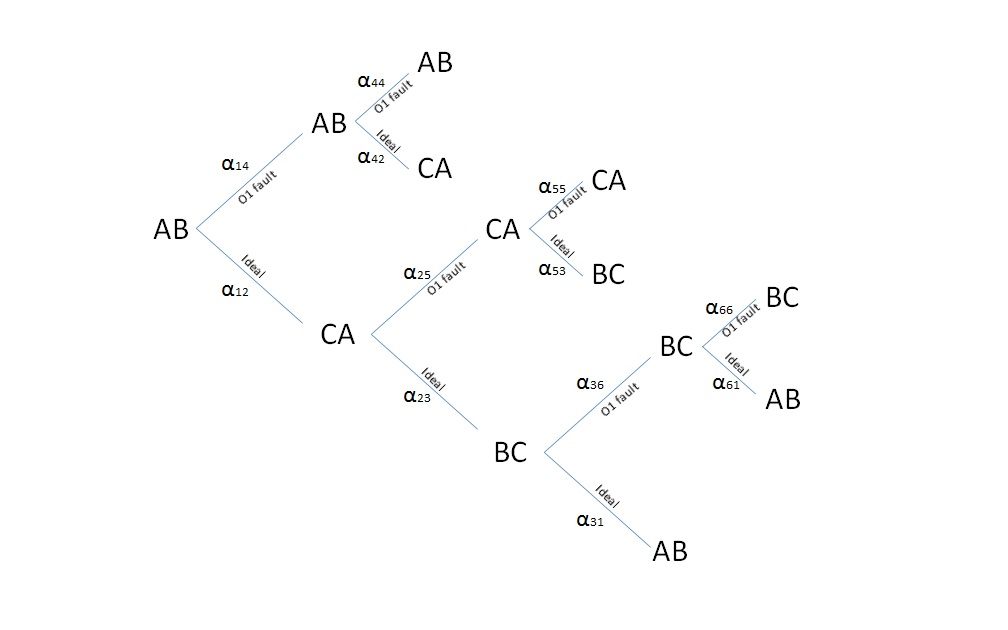
\includegraphics [width=4 in]{transitions.jpg}
\caption{\bf Possible layer transitions for LiNiO$_2$ containing O1-type stacking faults, where $\alpha_{ij}$ is the probability transition from layer \emph{i} to layer \emph{j}.}
\label{capes}
\end{center}
\end{figure}
 

\begin{sidewaysfigure}
\begin{center}
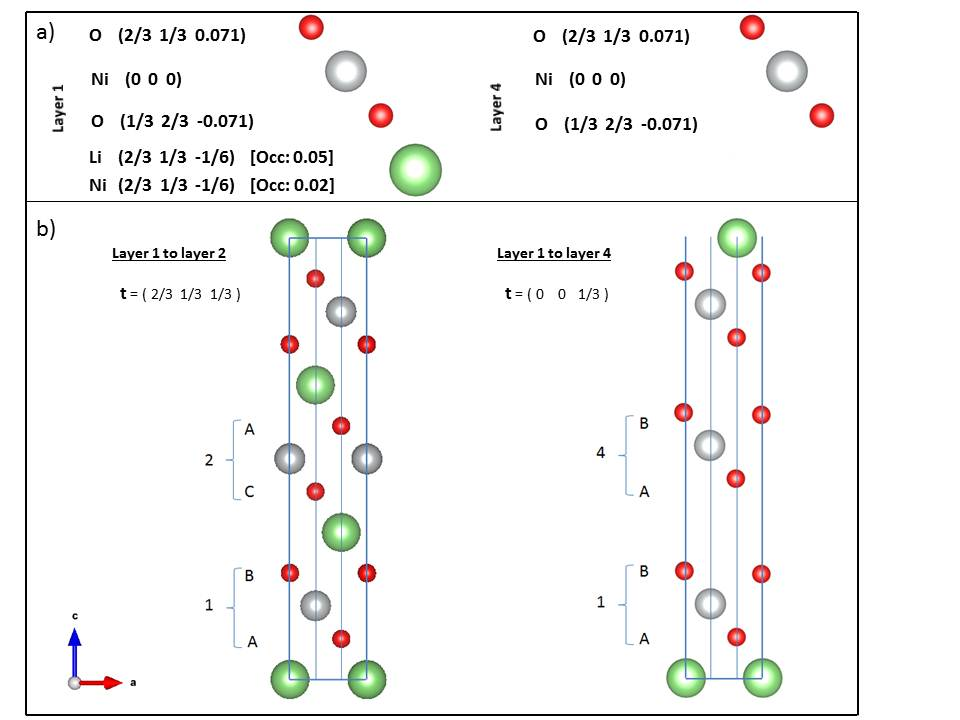
\includegraphics [width=6in]{description.jpg}
\caption{\bf  a) Schematic representation and atomic coordinates of the layers required for describing stacking faults for LiNiO$_2$ in the FAULTS program. b) Graphic representation of the different transition possibilities from layer 1 and transition vectors.}
\label{esquemacapes}
\end{center}
\end{sidewaysfigure}


\begin{table}
\begin{center}
\begin{tabular}{|c|c|c|c|}
\hline
Refined parameter & Simulation & Initial value & Final value \\
\hline
x & 0.600 & 0.700 & 0.604 \\
\hline
a,b & 2.8659 & 2.7868 & 2.8662 \\
\hline
c & 14.253 & 14.453 & 14.253 \\
\hline
x$_{Ni}$ & 0.000 & 0.200 & 0.004 \\
\hline
x$_{O}$ & 1/3 & 0.500 & 0.327 \\
\hline
z$_{Li}$ & 0.167	&0.267&	0.162 \\
\hline
$\alpha_{11}$ & 0.112&	0.142	&0.111\\
\hline
$\alpha_{12}$ & 0.888	&0.858&	0.889 \\
\hline
$\alpha_{22}$ & 0.112&	0.142	&0.111\\
\hline
$\alpha_{23}$ & 0.888	&0.858	&0.889 \\
\hline
$\alpha_{31}$ & 0.888&	0.858&	0.888 \\
\hline
$\alpha_{33}$ & 0.112&	0.142&	0.112\\
\hline

\end{tabular}
\caption{\textbf{Starting and final values of the parameters refined in the analysis of simulated data.}}
\label{taulasim}
\end{center}
\end{table}

\begin{figure}[!htbp]
\begin{center}
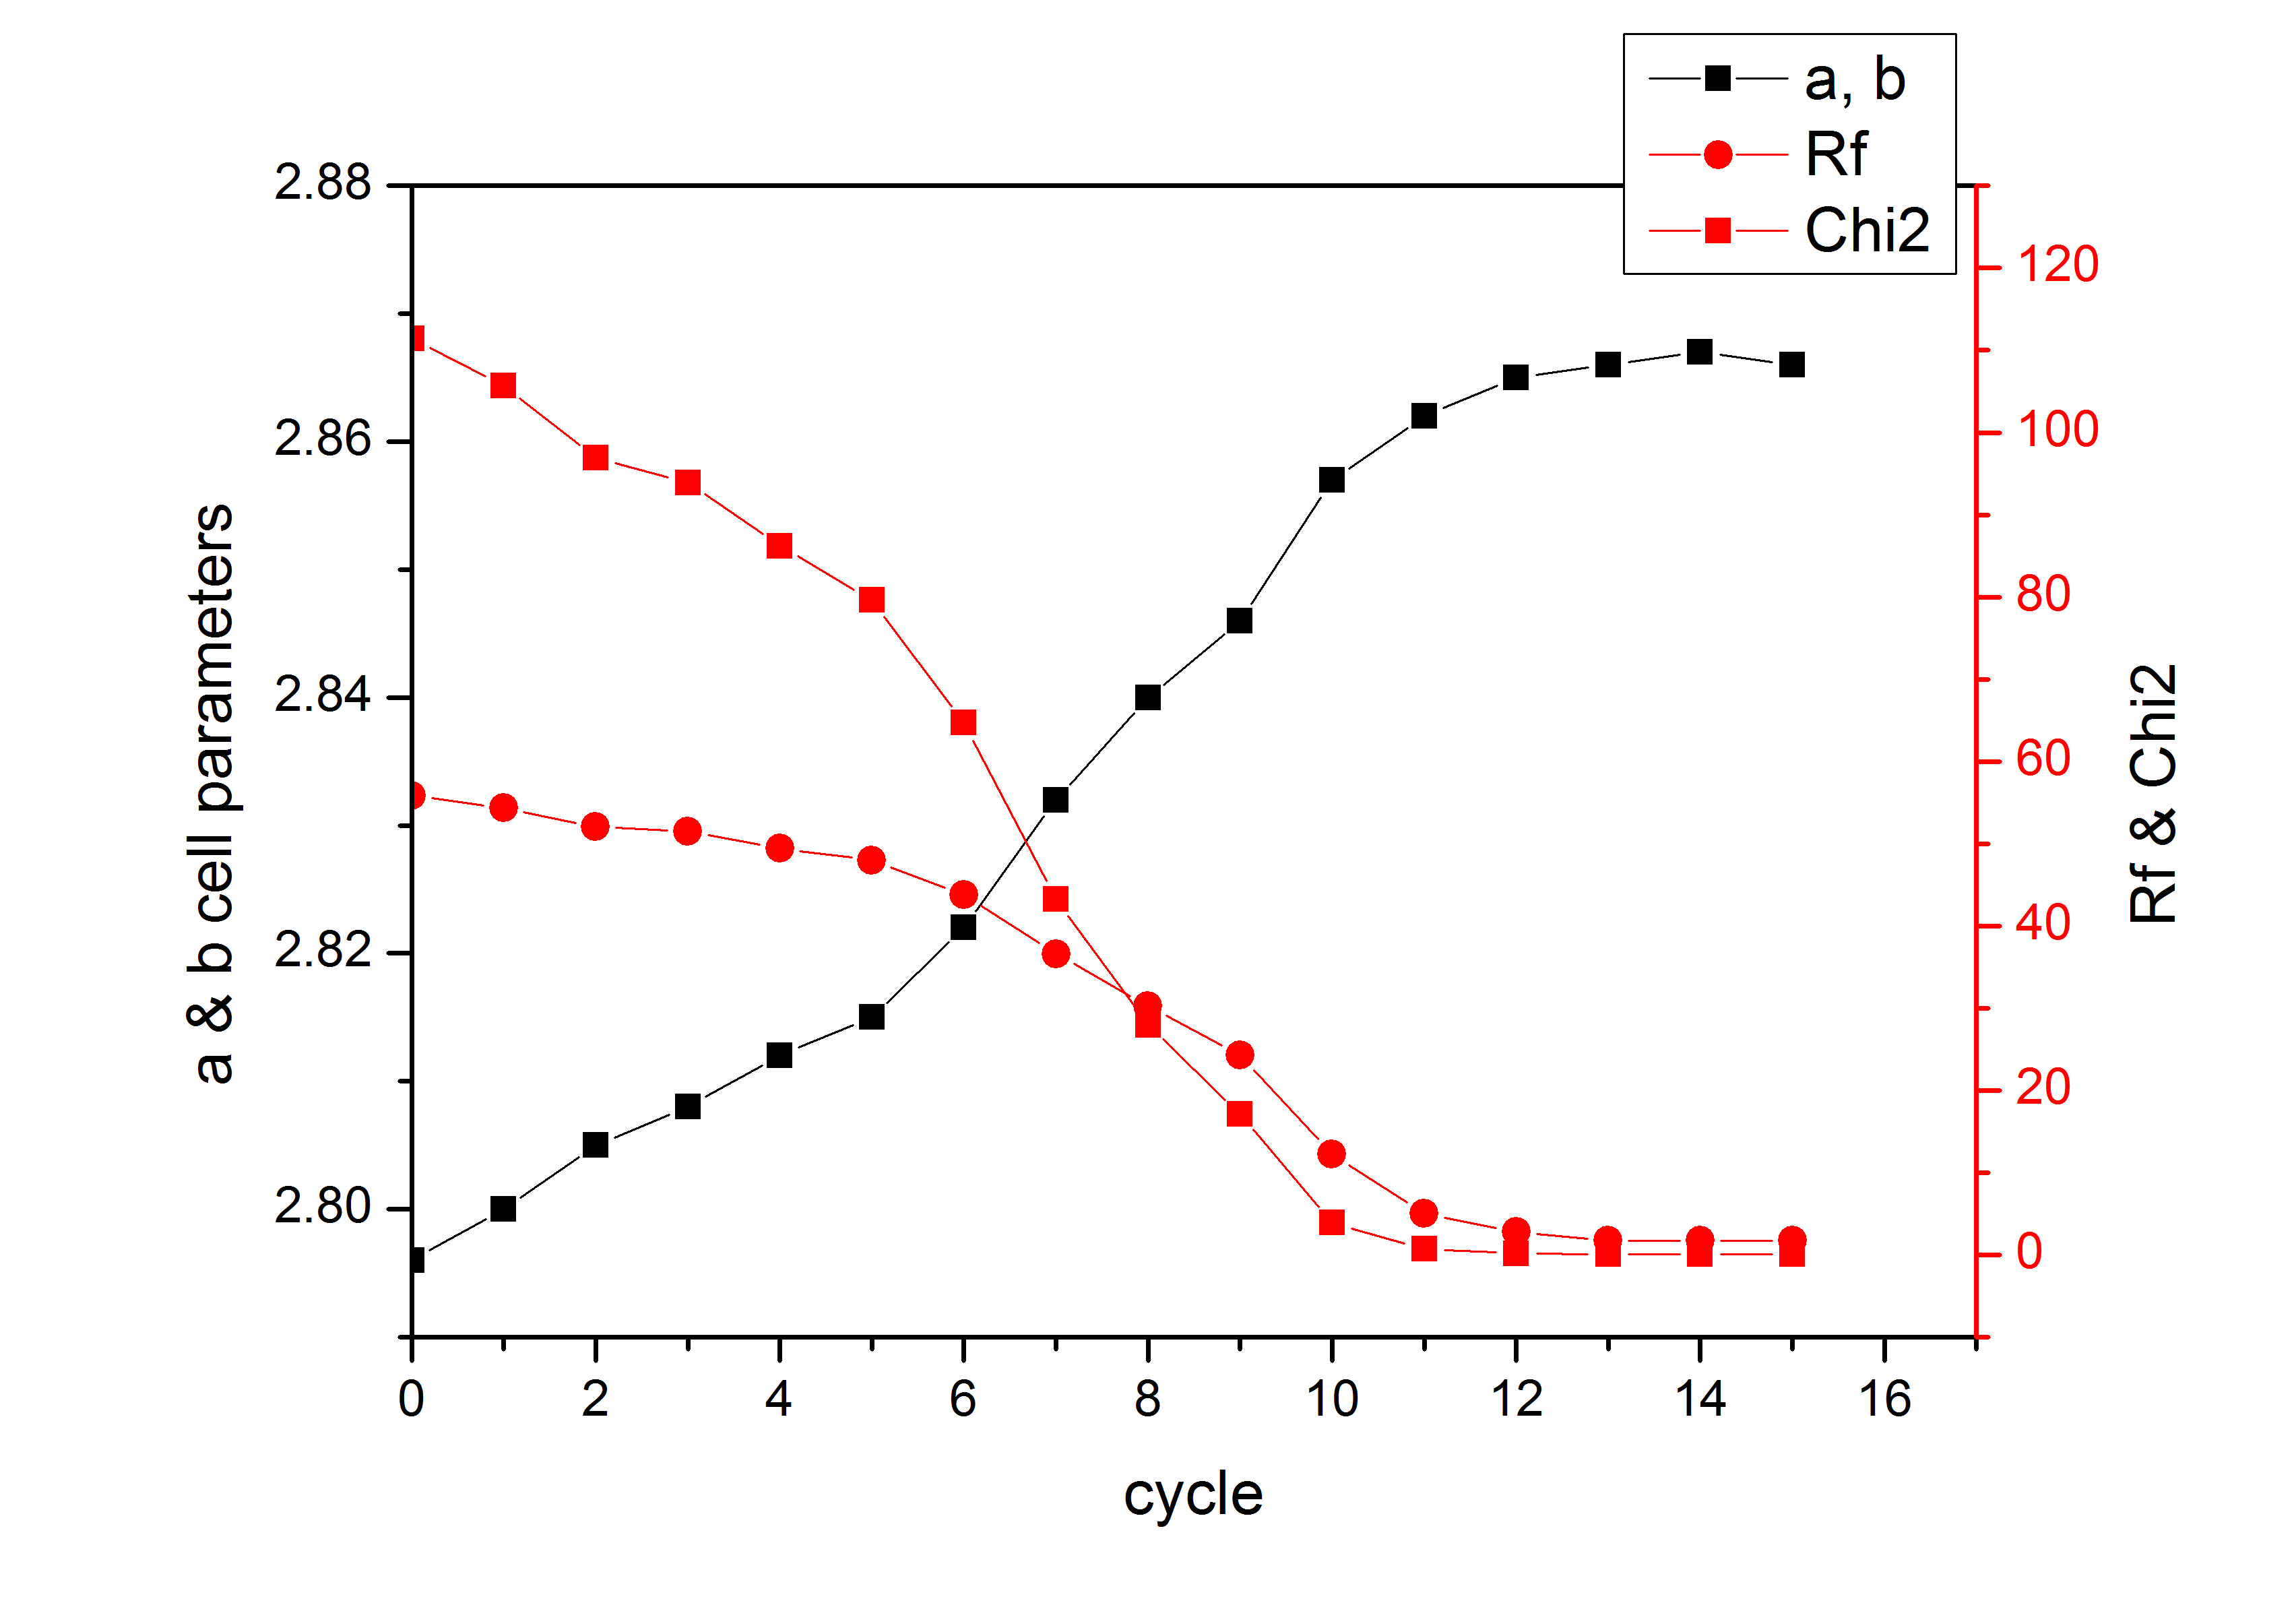
\includegraphics [width=4 in]{Rp_Chi2_ab_grafika_2.jpg}
\caption{\bf Evolution of the functions Rp and Chi$^{2}$ and of the cell parameters a and b, versus the cycle number. }
\label{cycles}
\end{center}
\end{figure}

\begin{sidewaysfigure}
\begin{center}
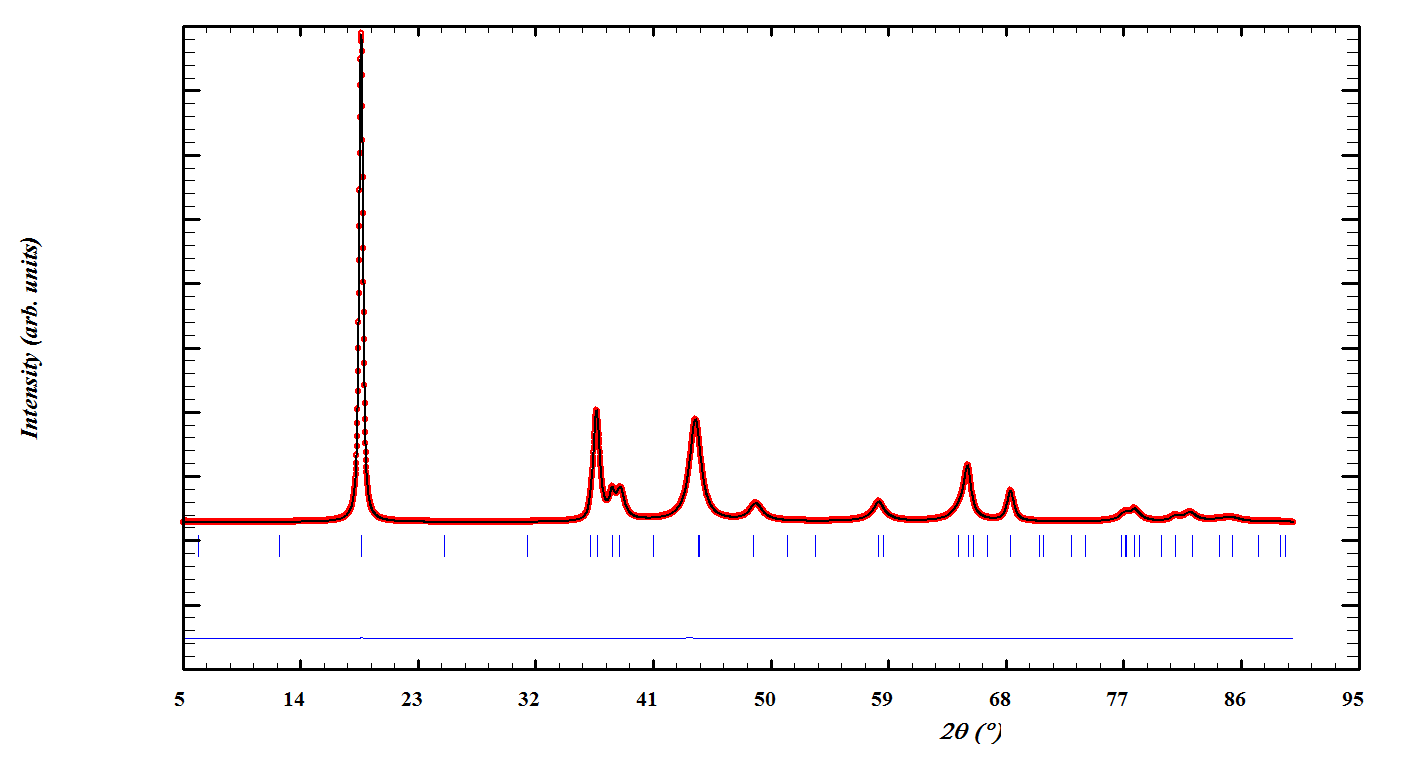
\includegraphics [width=6 in]{pattern.png}
\caption{\bf Comparison of the X-ray diffraction patterns corresponding to the FAULTS analysis of the simulated data: simulated pattern (dotted curve) and calculated pattern using the FAULTS refinement (continuous curve). The diagram underneath shows the difference between them.  }
\label{sim}
\end{center}
\end{sidewaysfigure}
